% Source: Code/ML_overlay/ir_rgb_registration/paper/ml_overlay_report_materials/ir_rgb_registration_report/figures/fig_regularization_effects.tex
\documentclass[tikz,border=10pt]{standalone}
\usepackage{tikz}
\usetikzlibrary{arrows.meta,positioning,calc,decorations.pathmorphing}

\definecolor{garnet}{RGB}{115,0,10}
\definecolor{rose}{RGB}{204,46,64}
\definecolor{atlantic}{RGB}{70,106,159}
\definecolor{congaree}{RGB}{31,65,77}
\definecolor{horseshoe}{RGB}{101,120,11}
\definecolor{black90}{RGB}{54,54,54}
\definecolor{black50}{RGB}{162,162,162}

\begin{document}
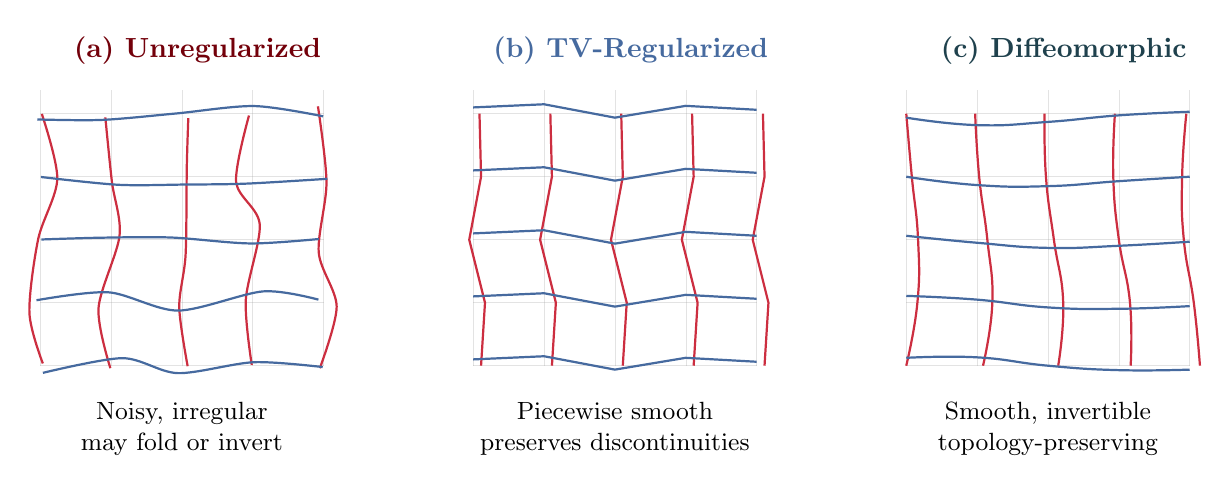
\begin{tikzpicture}[>=Stealth]

    % (a) Unregularized - noisy/folding grid
    \begin{scope}[local bounding box=unreg]
        \node[font=\bfseries, garnet] at (2,4) {(a) Unregularized};

        % Original grid (light)
        \foreach \i in {0,...,4} {
            \draw[black50, very thin, opacity=0.3] (\i*0.9,0) -- (\i*0.9,3.5);
            \draw[black50, very thin, opacity=0.3] (0,\i*0.8) -- (3.6,\i*0.8);
        }

        % Deformed grid with noise and folding
        \foreach \i in {0,...,4} {
            \draw[rose, thick]
                plot[smooth, tension=0.5] coordinates {
                    (\i*0.9+0.1*rand,0.05*rand)
                    (\i*0.9+0.2*rand,0.8+0.15*rand)
                    (\i*0.9-0.15*rand,1.6+0.2*rand)
                    (\i*0.9+0.25*rand,2.4+0.15*rand)
                    (\i*0.9+0.1*rand,3.2+0.1*rand)
                };
        }
        \foreach \i in {0,...,4} {
            \draw[atlantic, thick]
                plot[smooth, tension=0.5] coordinates {
                    (0.05*rand,\i*0.8+0.1*rand)
                    (0.9+0.15*rand,\i*0.8+0.15*rand)
                    (1.8+0.2*rand,\i*0.8-0.1*rand)
                    (2.7+0.15*rand,\i*0.8+0.2*rand)
                    (3.6+0.1*rand,\i*0.8+0.05*rand)
                };
        }

        \node[font=\small, text width=3.5cm, align=center] at (1.8,-0.8) {
            Noisy, irregular\\may fold or invert
        };
    \end{scope}

    % (b) TV-regularized - piecewise smooth
    \begin{scope}[shift={(5.5,0)}, local bounding box=tv]
        \node[font=\bfseries, atlantic] at (2,4) {(b) TV-Regularized};

        % Original grid (light)
        \foreach \i in {0,...,4} {
            \draw[black50, very thin, opacity=0.3] (\i*0.9,0) -- (\i*0.9,3.5);
            \draw[black50, very thin, opacity=0.3] (0,\i*0.8) -- (3.6,\i*0.8);
        }

        % Piecewise smooth deformed grid
        \foreach \i in {0,...,4} {
            \draw[rose, thick]
                (\i*0.9+0.1,0) --
                (\i*0.9+0.15,0.8) --
                (\i*0.9-0.05,1.6) --
                (\i*0.9+0.1,2.4) --
                (\i*0.9+0.08,3.2);
        }
        \foreach \i in {0,...,4} {
            \draw[atlantic, thick]
                (0,\i*0.8+0.08) --
                (0.9,\i*0.8+0.12) --
                (1.8,\i*0.8-0.05) --
                (2.7,\i*0.8+0.1) --
                (3.6,\i*0.8+0.05);
        }

        \node[font=\small, text width=3.5cm, align=center] at (1.8,-0.8) {
            Piecewise smooth\\preserves discontinuities
        };
    \end{scope}

    % (c) Diffeomorphic - smooth and invertible
    \begin{scope}[shift={(11,0)}, local bounding box=diffeo]
        \node[font=\bfseries, congaree] at (2,4) {(c) Diffeomorphic};

        % Original grid (light)
        \foreach \i in {0,...,4} {
            \draw[black50, very thin, opacity=0.3] (\i*0.9,0) -- (\i*0.9,3.5);
            \draw[black50, very thin, opacity=0.3] (0,\i*0.8) -- (3.6,\i*0.8);
        }

        % Smooth invertible deformed grid
        \foreach \i in {0,...,4} {
            \pgfmathsetmacro{\offset}{0.15*sin(\i*30)}
            \pgfmathsetmacro{\offseta}{0.2*sin(\i*30+45)}
            \pgfmathsetmacro{\offsetb}{0.15*sin(\i*30+90)}
            \pgfmathsetmacro{\offsetc}{0.1*sin(\i*30+135)}
            \pgfmathsetmacro{\offsetd}{0.05*sin(\i*30+180)}
            \draw[rose, thick]
                plot[smooth, tension=0.8] coordinates {
                    (\i*0.9+\offset,0)
                    (\i*0.9+\offseta,0.8)
                    (\i*0.9+\offsetb,1.6)
                    (\i*0.9+\offsetc,2.4)
                    (\i*0.9+\offsetd,3.2)
                };
        }
        \foreach \i in {0,...,4} {
            \pgfmathsetmacro{\offset}{0.1*cos(\i*30)}
            \pgfmathsetmacro{\offseta}{0.15*cos(\i*30+45)}
            \pgfmathsetmacro{\offsetb}{0.12*cos(\i*30+90)}
            \pgfmathsetmacro{\offsetc}{0.08*cos(\i*30+135)}
            \pgfmathsetmacro{\offsetd}{0.05*cos(\i*30+180)}
            \draw[atlantic, thick]
                plot[smooth, tension=0.8] coordinates {
                    (0,\i*0.8+\offset)
                    (0.9,\i*0.8+\offseta)
                    (1.8,\i*0.8+\offsetb)
                    (2.7,\i*0.8+\offsetc)
                    (3.6,\i*0.8+\offsetd)
                };
        }

        \node[font=\small, text width=3.5cm, align=center] at (1.8,-0.8) {
            Smooth, invertible\\topology-preserving
        };
    \end{scope}

\end{tikzpicture}
\end{document}
